\documentclass[conference]{IEEEtran}
\usepackage{graphicx}
\hyphenation{op-tical net-works semi-conduc-tor}
\usepackage{cite}
\begin{document}

\title{FARAZIST: Fast Automatic RVM And Zero-time Image Processing System}


% author names and affiliations
% use a multiple column layout for up to three different
% affiliations
\author{\IEEEauthorblockN{Sara Zarei}
\IEEEauthorblockA{Department of Computer Engineering\\
Islamic Azad University\\
Mashhad, Iran\\
Email: s.zarei@mshdiau.ac.ir}
\and
\IEEEauthorblockN{Amirmohammad Rouholamini\\ and Sajjad Aemmi}
\IEEEauthorblockA{Department of Computer Engineering\\
Ferdowsi University of Mashhad\\
Mashhad, Iran\\
Email: amirrouholamini@mail.um.ac.ir\\
sajjadaemmi@mail.um.ac.ir}
\and
\IEEEauthorblockN{Nasrollah Faramarzi}
\IEEEauthorblockA{Department of Computer Engineering\\
Tabran Higher Education Institute\\
Mashhad, Iran\\
Email: ceo@farazist.ir}}

% make the title area
\maketitle

\begin{abstract}
Plastic pollution is one of the most important environmental issues that various countries are facing it. More than eight million tons of plastic are released into the oceans each year and according to some estimates, by 2050, the number of plastics in the oceans will exceed the number of fish. So, the countries are looking for new ways to encourage people to recycle, especially recycling plastic waste. Reverse Vending Machine (RVM) is one of the popular methods that is being used by developed countries to help recycling. It accepts used beverage containers and returns money or ticket to the user. In this paper, we present a smart RVM system that collects the empty bottles (plastic, glass, aluminum, etc) and classifies them by using machine learning algorithm. After receiving the waste, this system recognizes the type of waste by machine learning algorithm based on python platform and pays a fee to user for the delivery. The accuracy of this  algorithm is 92\% on experimental images and 99\% on trained images. Implemented system shows that each bottle is recognized in 2.0 seconds. Our designed RVM can be developed for other types of waste.
\end{abstract}

% no keywords


\IEEEpeerreviewmaketitle


\section{Introduction}
% no \IEEEPARstart
Environmental pollution caused by waste is one of the most important issues in today's world and various countries are facing it. Each year, more than eight million tones of plastic end up in the oceans and costing at least eight billion dollars in damage to marine ecosystems. According to some estimates, by 2050 oceans will carry more plastic than number of fish and an estimated 99\% of seabirds will have ingested plastic \cite{jakovljevic2020deep}\cite{2020u}.
\par
Polyethylene Terephthalate (PET) is the most widely produced and recycled plastic that consumed in industrial and residential areas because of its great properties such as low cost, impact strength, and etc\cite{zhang2020pet}. It is important to create methods that encourage people to recycle. RVM is one of the incentive ways to collect and recycle plastic bottles. It takes in used scraps such as plastic bottles and changes them to money or ticket\cite{sambhi2020reverse}. RVM consists of an electronic circuits system and a doorway that directs a bottle to a bottle storage place. In this machine, sensors detect the entry and exit of bottles and the type of each bottle is recognized by machine learning algorithms.
\par
In this article, we introduce the smart RVM called FARAZIST that can recognize all types of glass, paper and aluminum bottles in addition to plastic bottles by artificial intelligence algorithms. Furthermore, our designed RVM can be implemented for other types of waste. To use FARAZIST, people need to create an account in the mobile application. Then, in addition to recycling items, they can use other services such as charging a residential unit, insurance payment, assistance to charity organizations, aid to environmental protection organizations, and etc. FARAZIST device can be managed with the mobile application. To facilitate further research, we have made our source publicly available \footnote{\url{https://github.com/Farazist/farazist-raspberrypi-app}}.
\par
The remainder of this paper is organized as follows: Section II introduces the related work and the proposed approach is introduced in section III. Section IV concludes the paper and finally, section V provides direction for future research.


\section{Related Work}
A RVM is a device that encourages people to recycle objects by receiving wastes and returning money to people. This device can recognize the type of wastes by using some techniques such as image processing. Although various RVMs were built, most of them only processed one type of waste. In the following section, we will examine several automatic waste delivery devices.
\par
In \cite{dhulekar2018development}, Dhulekar et al, proposed new design for RVM called Bottle Recycling Machine (BRM) to collect plastic bottles and aluminum cans to provide an efficient waste collection system. They classified these bottles using deep learning techniques. A camera takes images of bottles and delivers them to the machine as input and a processor tells whether it is bottle or not. They use  Raspberry Pi model B as a processor unit which is responsible for bottle identification and then controls the input and output of the sensors based on its diagnosis. Then, signals from all these sensors are given to the processing system. They used a Human Machine Interface (HMI) that included an LCD and voice instructions to connect users to the device. Using the servo motor, BRM can put bottles in the respective compartment after identification. A thermal printer is used to give the user a reward coupon and Real-Time Clock (RTC) is required to display and print date and time on coupon. Images taken from the camera are given to the Convolutional Neural Networks (CNN) to extract the relevant features and make the classification. They use supervised learning to train classifiers to classify objects. In this article, training of a classifier is done with the TensorFlow library. BRM takes 7.0 to 9.0 seconds to identify the bottle with an accuracy of 80\% to 100\%.
\par
Ziouzios et al, in \cite{ziouzios2019smart} designed a smart recycling bin using modern methods to classify waste. This machine consists of two partitions: a waste entry area on the top and an identification unit which features an electromechanically controlled seal on the bottom. By pressing the enter button, a camera captures a frame of the identification unit and the seal is opened in order to empty the unit. Then, the system performs the recognition of the waste. This system is based on ARM embedded devices including the Raspberry Pi 3 and the Xilinx Pynq-Z1 FPGA board. The authors of this paper use CNN to classify six classes, including 2,527 images of cardboard, glass, metal, paper, plastic or trash. Their model classified waste with an accuracy of 92.1\% on the test data.\par

In \cite{mwangi2019using}, Wanini Mwangi et al, established mechanisms to identify the status of PET bottles after the consumer for recycling. In this research, different types of PET in four classes seal, cap, seal & cap, no seal, and cap content were examined and a total of 1749 images were captured by Raspberry Pi camera. They used Squeeze Net as deep learning technology to train the PET bottles images and they reached 98\% accuracy with correct bottle status recognized. They deployed their model on a Raspberry Pi 2 model B to detect PET bottles in real time when using a RVM. They also used range sensor (HC-SR04) to detect the bottle which triggers the camera to take photos. By measuring prediction performance, this model showed a delay of 0.1 to 0.25 seconds per prediction using raspberry pi CPU.\par

Adedeji et al,\cite{adedeji2019intelligent} proposed a waste classification system based on CNN model called ResNet-50. The authors used  Support Vector Machine (SVM) to classify the waste into different groups and they were able to classify them with 87\% accuracy. The data set used in this article includes the 1989 image with size 512 × 384 in 4 classes: plastic, glass,  metal, and paper.

\section{Proposed approach}
In the proposed design of RVM, bottle identification is done by the use of machine learning. The model is trained to identify 40 classes of bottles. An Image of a bottle is given to the RVM machine as input and then this system then identifies the class and the kind of the bottles. In the following section, we will explain our proposed system in four groups: software, deep learning, hardware, and system flow design.

\subsection{Software}
Our RVM application called FARAZIST is a python based application that is developed on python 3.7. This system is compiled and implemented on Raspberry Pi OS (which is a Debian-based operating system for Raspberry Pi) \cite{2020raspberry}. In this RVM device, some information, such as General Purpose Input/Output (GPIO) pin numbers of press motor, distance sensors, separation motor, and conveyor motor are stored on the local SQLite database. For designing the main server and database PHP language, Laravel framework and MySQL are used. All private and important values are encrypted using OpenSSL and the AES-256-CBC cipher algorithm.\par

\subsection{Deep Learning}
We trained a CNN to classify bottle images into different classes. Details are provided below: 

\subsubsection{Dataset}
Our dataset consists of more than 5000 high resolution images from 40 classes which have variable resolutions, while our system requires a constant input dimensionality. Therefore, we reduced the images size to a fixed resolution of 320x320x3. We did not pre-process the images in any other way, except for scale pixel values of RGB images in range 0 and 1 as normalization.

\subsubsection{Data Augmentation}
The accuracy and performance of deep learning neural networks are often enhanced with increasing the number of training images in dataset. Data augmentation is a technique to artificially create new training data from existing training data. This is done by applying domain-specific techniques to examples from the training data that create new and different training examples.
\par 
Image data augmentation is perhaps the most well-known type of data augmentation and involves creating transformed versions of images in the training dataset that belong to the same class as the original image. Transforms include a range of operations from the field of image manipulation, such as shifts, horizontal flip, vertical flip, width shift, height shift, brightness, shear, rotation, zooms, and much more. Figure 1 shows an augmentation examples for aluminum cans.

\begin{figure}[h!]
    \footnotesize
	\centering
    \begin{tabular}{c c c}
    \subfloat{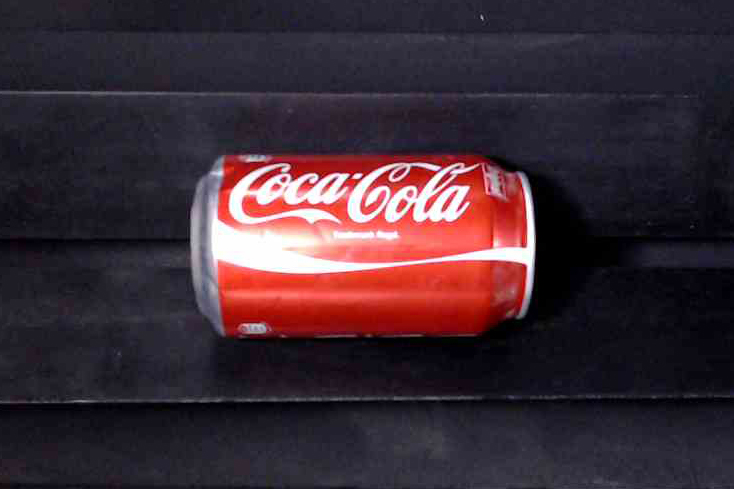
\includegraphics[width = 1in]{6.jpg}} &
    \subfloat{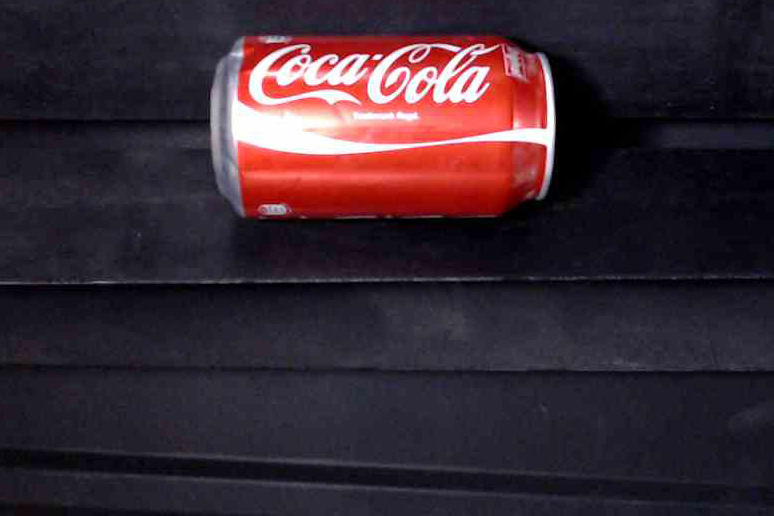
\includegraphics[width = 1in]{5.jpg}} &
    \subfloat{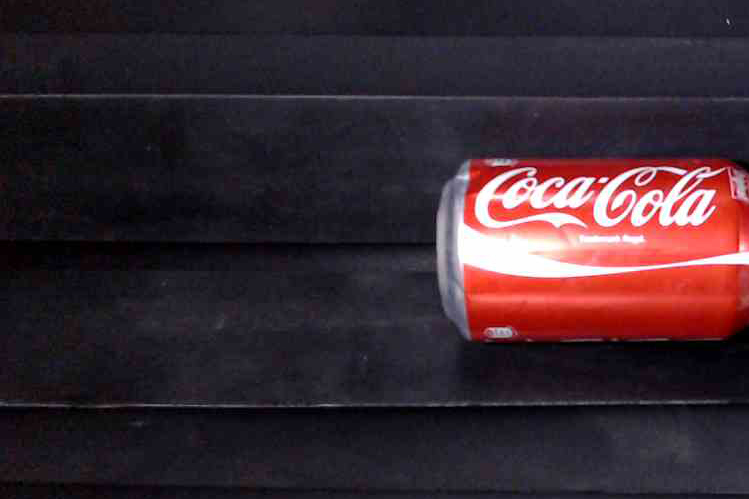
\includegraphics[width = 1in]{4.jpg}} &\\
    (a) & (b) & (c)\\[2ex]
    \subfloat{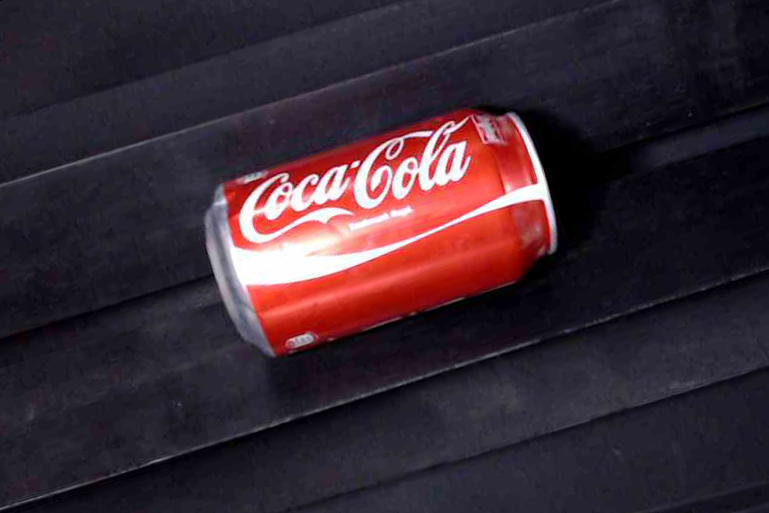
\includegraphics[width = 1in]{3.jpg}} &
    \subfloat{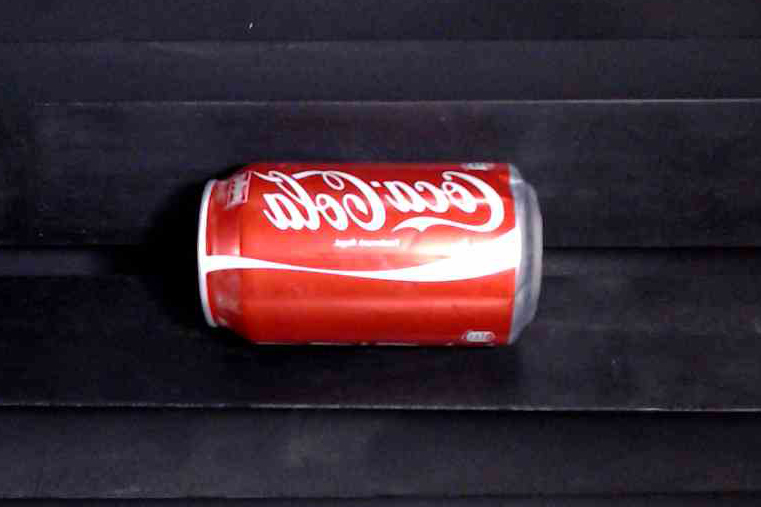
\includegraphics[width = 1in]{2.jpg}} &
    \subfloat{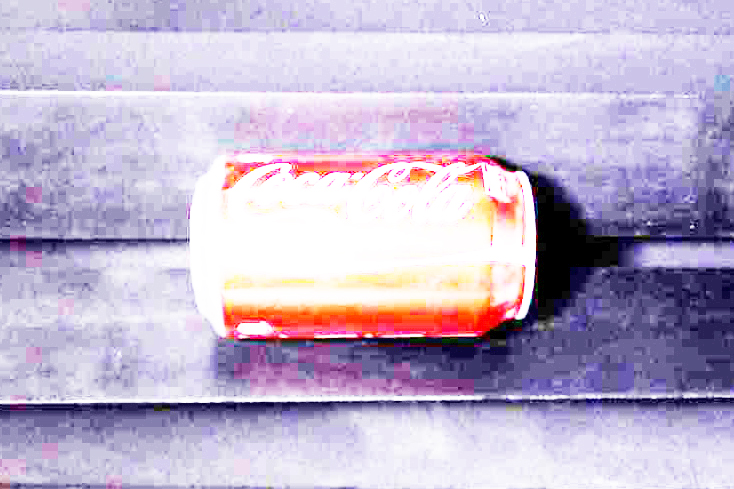
\includegraphics[width = 1in]{1.jpg}} &\\
    (d) & (e) & (f)\\[2ex]
    \end{tabular}
    \caption{Augmentation examples, a: input image, b: height shift, c: width shift, d: shear, e: horizontal flip, f: brightness}
\end{figure}

\subsubsection{Frameworks}
TensorFlow selected as main framework for deep learning part of FARAZIST project. TensorFlow is an end-to-end open source platform for machine learning \cite{2020t}\cite{abadi2016tensorflow} which is used to train CNN for object detection and image classification. We also have used other libraries like SciPy, OpenCV, Keras, and etc to train, evaluate and predict our deep neural network model and implement the software. \par
We have used TensorFlow GPU for training CNN. Then, we saved trained model and converted it to tflite file. Tflite is lite edition of TensorFlow that is optimized for on-device inference on mobile, embedded, and IoT devices \cite{tensorflow-lite}. It enables on-device machine learning inference with low latency and a small binary size. TensorFlow Lite is designed to make it easy to perform machine learning on devices "at the edge" of the network instead of sending data back and forth from a server.

\subsubsection{Network Architecture}
We have used SSD\footnote{Single Shot Detector} and MobileNetV2 \cite{s2018mobilenetv2} architecture to feature extraction, object detection and classify images. MobileNet is a CNN model and has 5.3 million parameters. Like other CNNs, this network consists of convolutional layers, some of which are followed by max-pooling layers, and one fully-connected layer with a final 40-way softmax based on number of dataset classes.
\pre
To reduce over fitting in the fully-connected layer, we employed a regularization term called “dropout” that proved to be very effective. Categorical-Crossentropy have been used for loss function.
Figure 2 shows the MobileNet and SSD architecture.

\begin{figure}
    \centering
    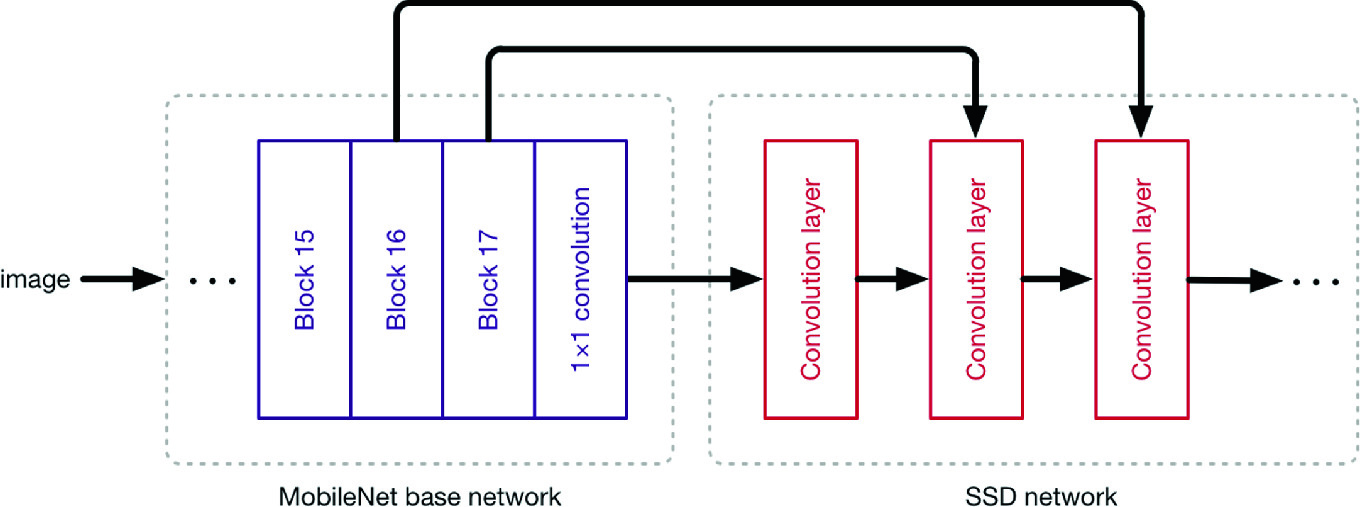
\includegraphics[width=0.45\textwidth]{mobilenet-ssd.png}
    \caption{MobileNet + SSD architecture}
\end{figure}

\subsubsection{Optimizer}
Adadelta optimization is a stochastic gradient descent method that is based on adaptive learning rate per dimension to address two drawbacks:

\begin{itemize}
  \item The continual decay of learning rates throughout training,
  \item The need for a manually selected global learning rate.
\end{itemize}\par

Adadelta is a more robust extension of Adagrad that adapts learning rates based on a moving window of gradient updates, instead of accumulating all past gradients. This way, Adadelta continues learning even when many updates have been done. Compared to Adagrad, in the original version of Adadelta you don't have to set an initial learning rate. In this version, initial learning rate can be set, as in most other Keras optimizers.
\par
Near the end of training step sizes are converged to 1 which are effectively a high learning rate which would cause divergence. This occurs only near the end of the training as gradients and step sizes are small, and the epsilon constant in the numerator and denominator dominate past gradients and parameter updates which are converge the learning rate to 1 \cite{zeiler2012adadelta}.

\subsubsection{Learning Details}
We trained our model with a batch size of 32 examples, Adadelta optimizer parameters for learning rate, rho and epsilon are 0.001, 0.95, and 1e-07 respectively. We found that this small amount of epsilon was important for the model to learn. To make training faster, we used ImageNet initial weights. On the test data, we achieved top-1 and top-5 accuracy rates of 71.3\% and 90.0\%, and 99\% on trained images. 
\par
We trained the network for roughly 80 cycles through the training set of 5000 images which took half a day on NVIDIA Tesla K80 580 12GB GPU. Figure 3 shows the accuracy and loss during the training our model.

\begin{figure}[h!]
    \footnotesize
	\centering
    \begin{tabular}{c c}
    \subfloat{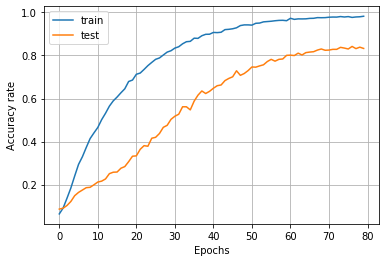
\includegraphics[width=0.22\textwidth]
    {accuracy.png}} &
    \subfloat{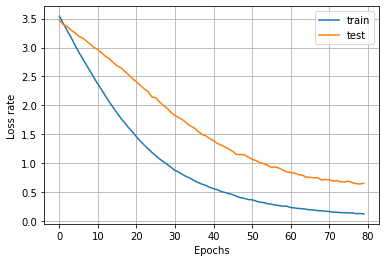
\includegraphics[width=0.22\textwidth]
    {loss.png}} &\\
    (a) & (b)\\[2ex]
    \end{tabular}
    \caption{This plot shows the accuracy (a) and  loss (b) on our train (blue line) and test (orange line) dataset for 80 epochs}
\end{figure}

\subsection{Hardware}
Figure 4 shows RVM architecture. In this system, the Raspberry Pi 4 model B is used as the main computer. Two distance sensors are used at the beginning and end of the conveyor belt to detect the entry and exit of bottles. When the first sensor detects the entry of the bottle, the conveyor belt turns on and the bottle moves inwards. Then, the bottle moves between the first and second sensors, and the camera starts imaging in 30 frames per seconds. we use Picamera NoIR v2 to do this. As soon as the second sensor detects the bottle, the conveyor belt turns off and a separation motor and press motor starts working to compress the bottle. {\color{red}This process takes about 5 seconds per bottle.}
\par
Raspberry Pi GPIO pins have been used to receive and send information to the Raspberry Pi. Since Raspberry Pi GPIP pins generate 5V power and 220V power is required to start the conveyor motors, press motor and separation motor, we have used the relay to convert the 5V to 220V power supply.
\par
A touch screen LCD has been used to facilitate communication between users and the RVM device. After logging in to the device and selecting the bottle delivery section, users can see the number, type of bottle and the cost that is paid to them for bottle delivery.

% add flow chart
\begin{figure}[h!]
  \centering
  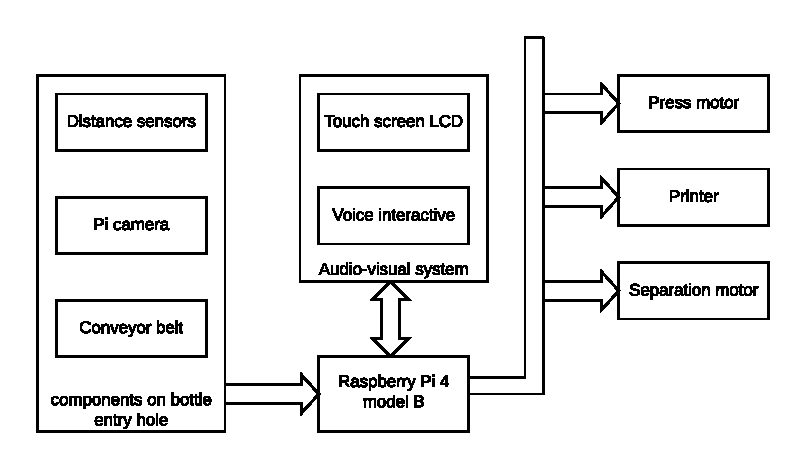
\includegraphics[width=0.5\textwidth]{fig1}
  \caption{Architecture of RVM}
\end{figure}
% add flow chart
\begin{figure}[H!]
  \centering
  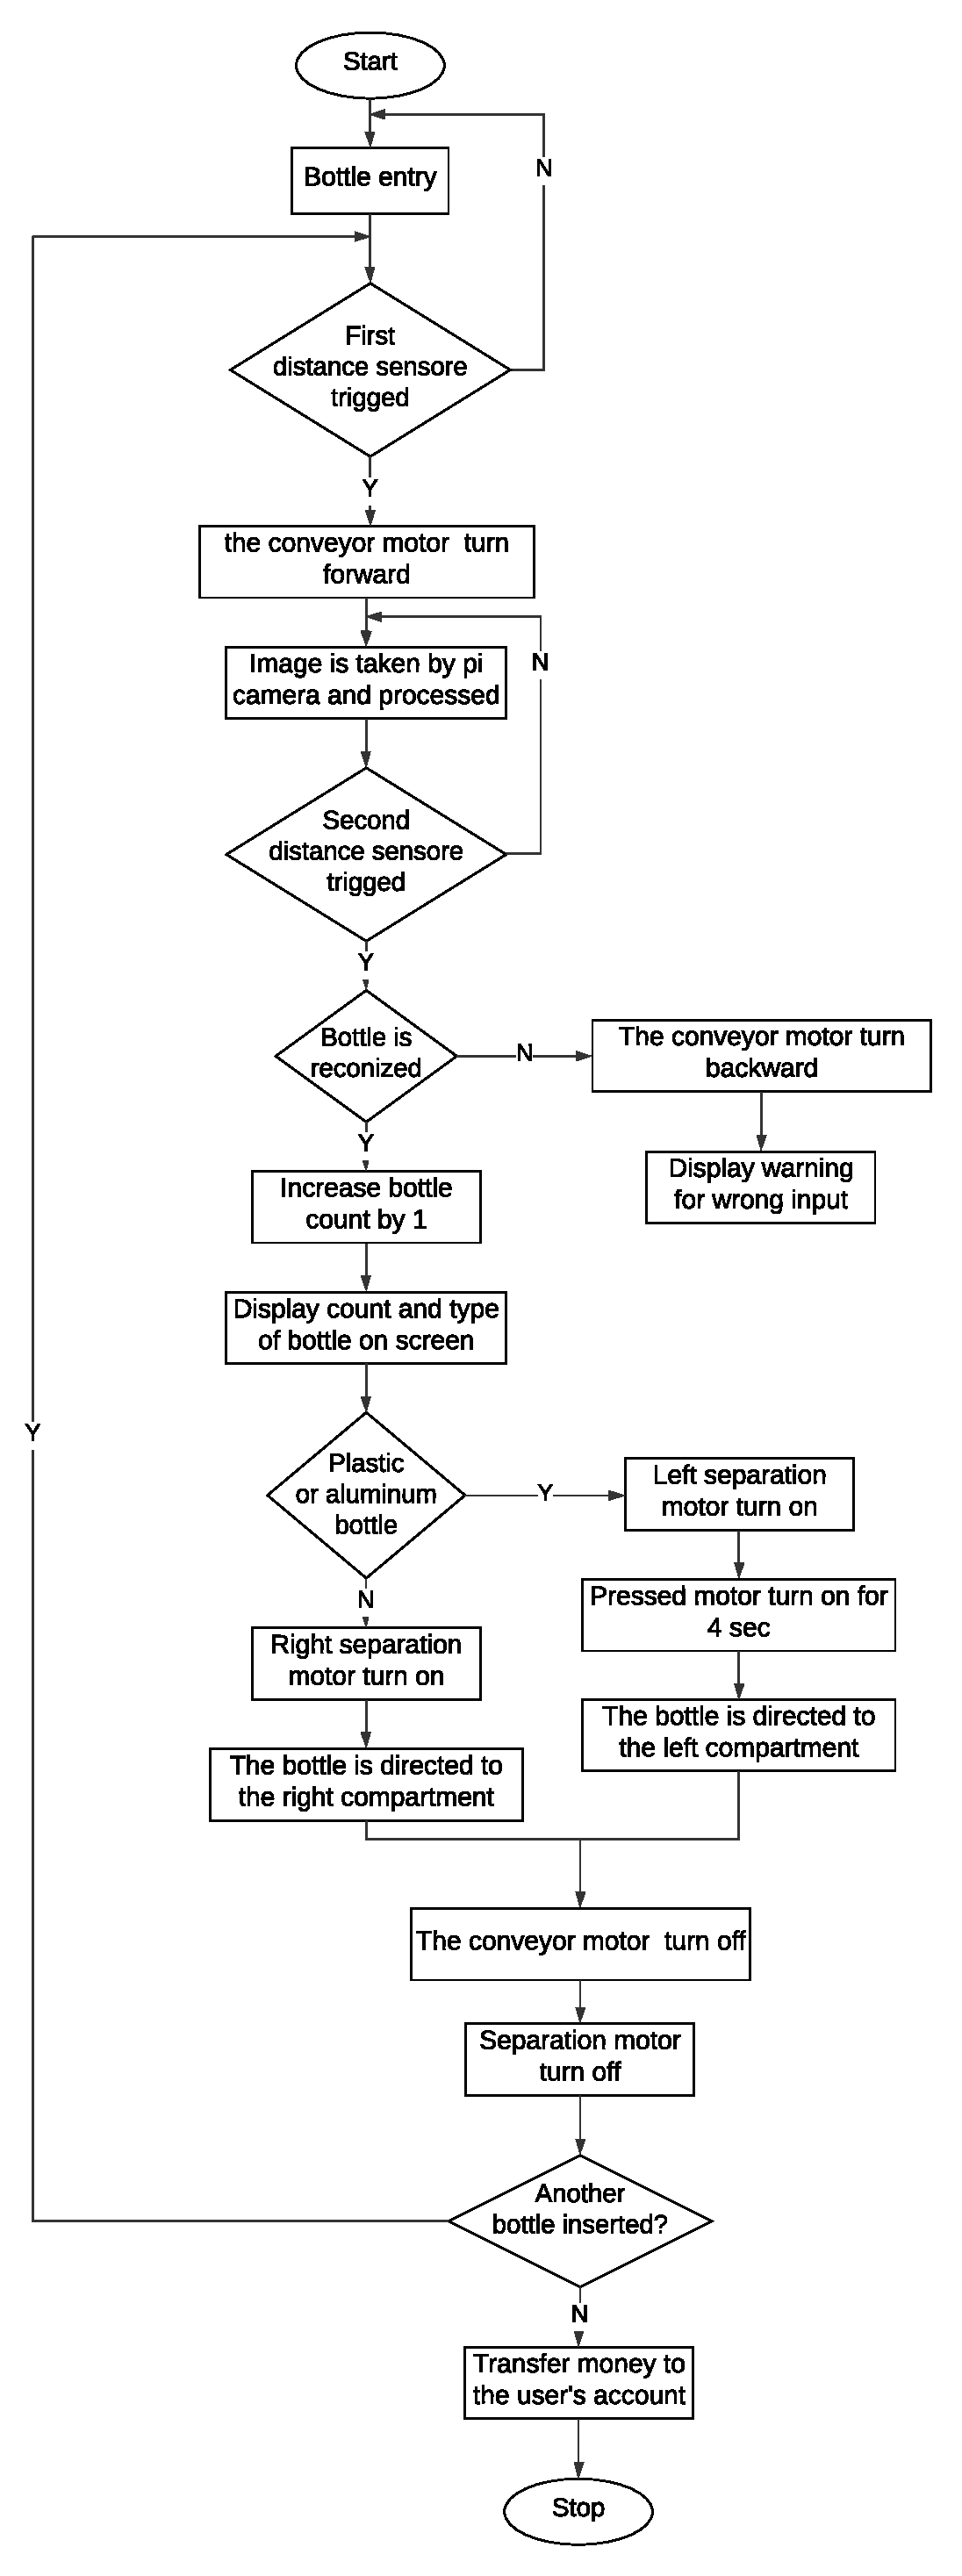
\includegraphics[width=0.5\textwidth]{fig2}
  \caption{Flow-chart of RVM operation}
\end{figure}

\subsection{System Flow Design}
\par 
A flowchart of RVM recycling bottle operation is given in Figure 5. First of all, you need to login to the RVM application with QR code or ID and password, and its requirement is that you have already created an account in the FARAZIST mobile application. The QR code used in the FARAZIST is generated by the server and displayed on the LCD, by scanning it, the user can connect to her/his own account. After that, to recycling the bottle(s), you must select the bottle delivery option from the main menu of the program.
\par 
When the bottle enters and the first sensor detects the entry of it, the conveyor motor turns on and the bottle moves inwards. Then, the bottle moves between the first and second sensors and the Pi Camera takes several images of it until the second sensor senses the bottle. In the next step, the images taken from the bottle are processed and if the designed model that was described in the previous sections cannot recognize it, conveyor belt moves in the opposite direction and takes out the bottle. Also, a warning message is displayed on the screen for the user to notice and take the bottle. But if the model can recognize the bottle, the cost of the bottle will be appeared on the LCD screen, and a message about recycling the bottle from the speaker is playing. Also, the user can see the name and number of bottles detected on the LCD. Figure 6 shows an overview of the proposed RVM, including the bottle entry section and the display.
\par 
In this device, we have used two separate compartments to store bottles after recycling: one compartment for plastic and aluminum bottles and one for other bottles. If the recognized bottle is plastic or aluminum, the separation motor directs them to the left chamber, and before being stored at this location, these bottles are pressed by the press motor. If the bottles are not plastic or aluminum, the separation motor will direct them to the right compartment. After that, separation and conveyor motors are turned off. In the last step, all the money is transferred to the user's virtual wallet.
%خلاصه ای از قابلیت های دیگه دستگاه

\begin{figure}
    \centering
    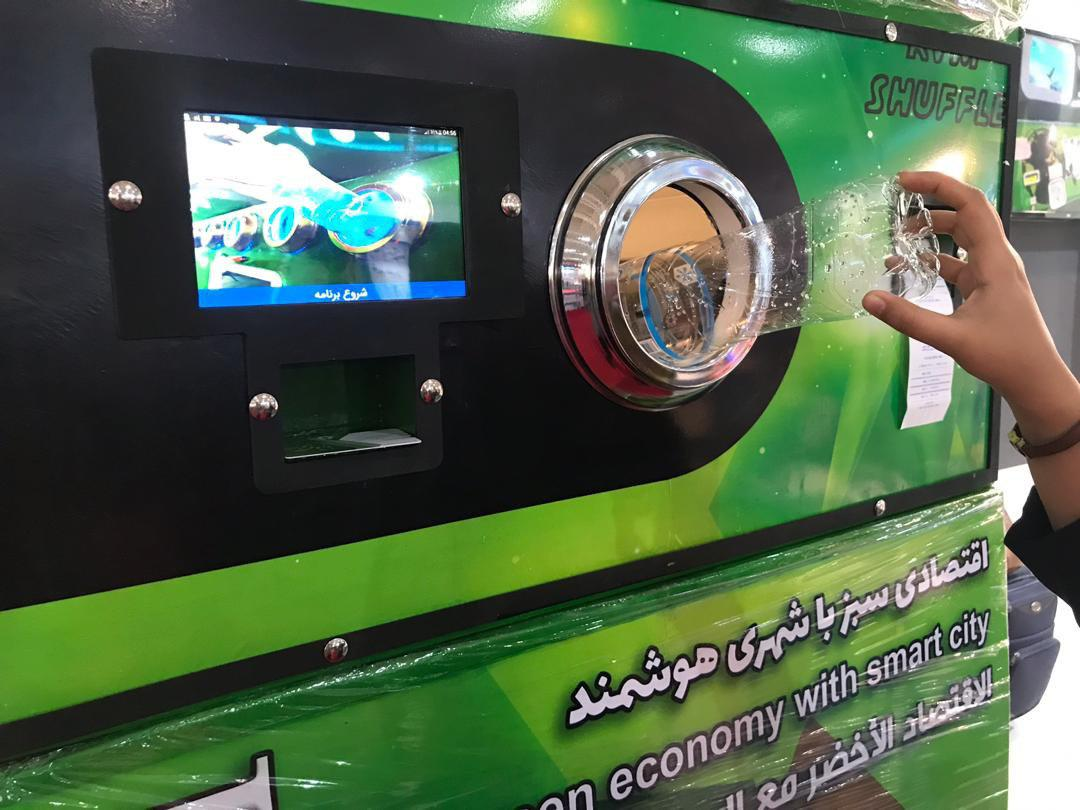
\includegraphics[width=0.5\textwidth]{RVM.jpg}
    \caption{A picture of RVM device.}
\end{figure}

\section{Conclusion}
Today, environmental pollution and mass production of plastic waste have become one of the most important environmental issues. In this paper, we present RVM, a smart reverse vending machine that in return for receiving empty bottles, it provides some services to its users or adds money to their virtual wallets. The RVM that we designed can recognize the type of bottle using image processing algorithms and the TensorFlow library. By using deep CNN, we classified bottles in 40 different classes. Our results showed that a small neural network such as NASNetMobile has the ability to categorize bottles well. We used the initial weights of ImageNet to train our model and were able to achieve accuracy 92\% on experimental data.

\section{Future Work}
In future work, we will design a mechanism for exiting bottles that are not recognized. In this design, the bottles that have not been recognized by the artificial intelligence model will be directed outward of the device through a special path. This increases the speed of the device proceed and does not require the user or operator to take unidentified bottles. In addition, we are looking to improve the bottle recognition algorithm. So, that with each new class of bottle added to the model, there is no need to train the model again.\par


% that's all folks
\bibliographystyle{unsrt}
\bibliography{reference}
\end{document}


